\chapter{Implementation and Functional Capabilities}
\label{ch:implementation}

This chapter details the functional capabilities of the CHOYXONA.UZ application across three user roles: customers, establishment administrators, and platform super administrators.
It covers the authentication and profile management module, the search-to-booking user journey, the administrator management dashboard, the super administrator platform oversight panel, and the notification system.
Each section includes screenshots from the implemented application demonstrating the described functionality.


% =====================================================================
\section{User Module: Registration and Authentication}
\label{sec:user-module}

The user module handles identity management throughout the application lifecycle, from initial registration through ongoing profile maintenance.
This foundational module ensures secure access to features while maintaining a frictionless onboarding experience~\cite{firebase_auth2024}.

\subsection{Authentication Methods}
\label{subsec:auth-methods}

CHOYXONA.UZ supports two primary authentication methods aligned with Uzbek user preferences:

\textbf{Email and password registration} provides the traditional account creation flow.
Users enter their email address, create a password meeting minimum complexity requirements (at least eight characters with mixed case and numbers), and confirm the password.
Upon successful registration, a verification email is sent, though the application permits limited functionality before verification to reduce onboarding friction~\cite{firebase_auth2024}.

\textbf{Phone number authentication} employs SMS-based one-time passwords (OTP).
Users enter their phone number in international format and receive a six-digit verification code via SMS.
This method is particularly relevant for the Uzbek market where phone numbers serve as primary identifiers~\cite{khawas2018}.

The application startup and authentication flow is illustrated in \cref{fig:splash-auth}.

\begin{figure}[htbp]
  \centering
  \begin{minipage}[b]{0.3\textwidth}
    \centering
    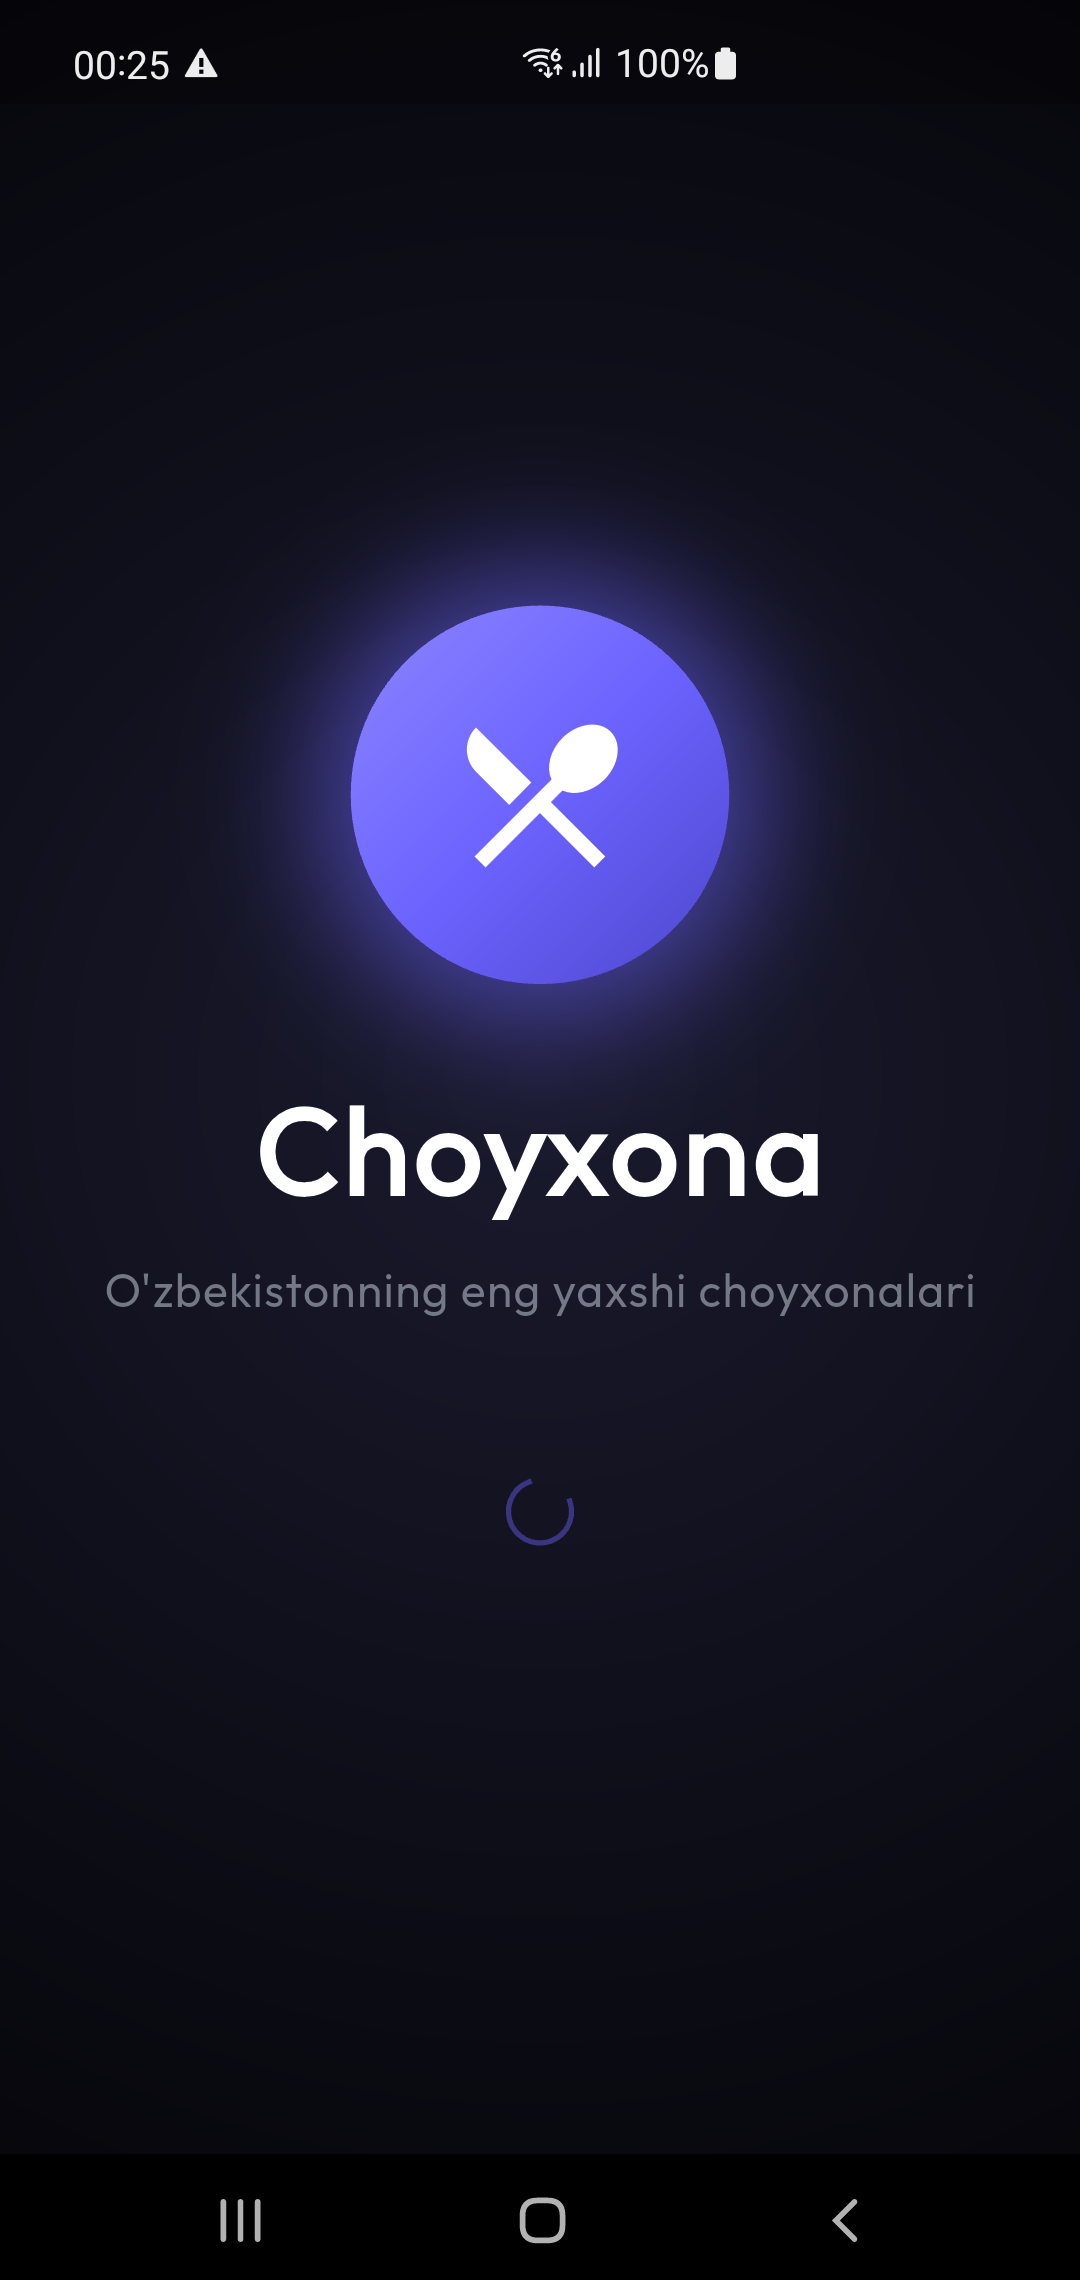
\includegraphics[width=\textwidth]{b_chapters/chapter3/assets/splash_screen.png}
  \end{minipage}
  \hfill
  \begin{minipage}[b]{0.3\textwidth}
    \centering
    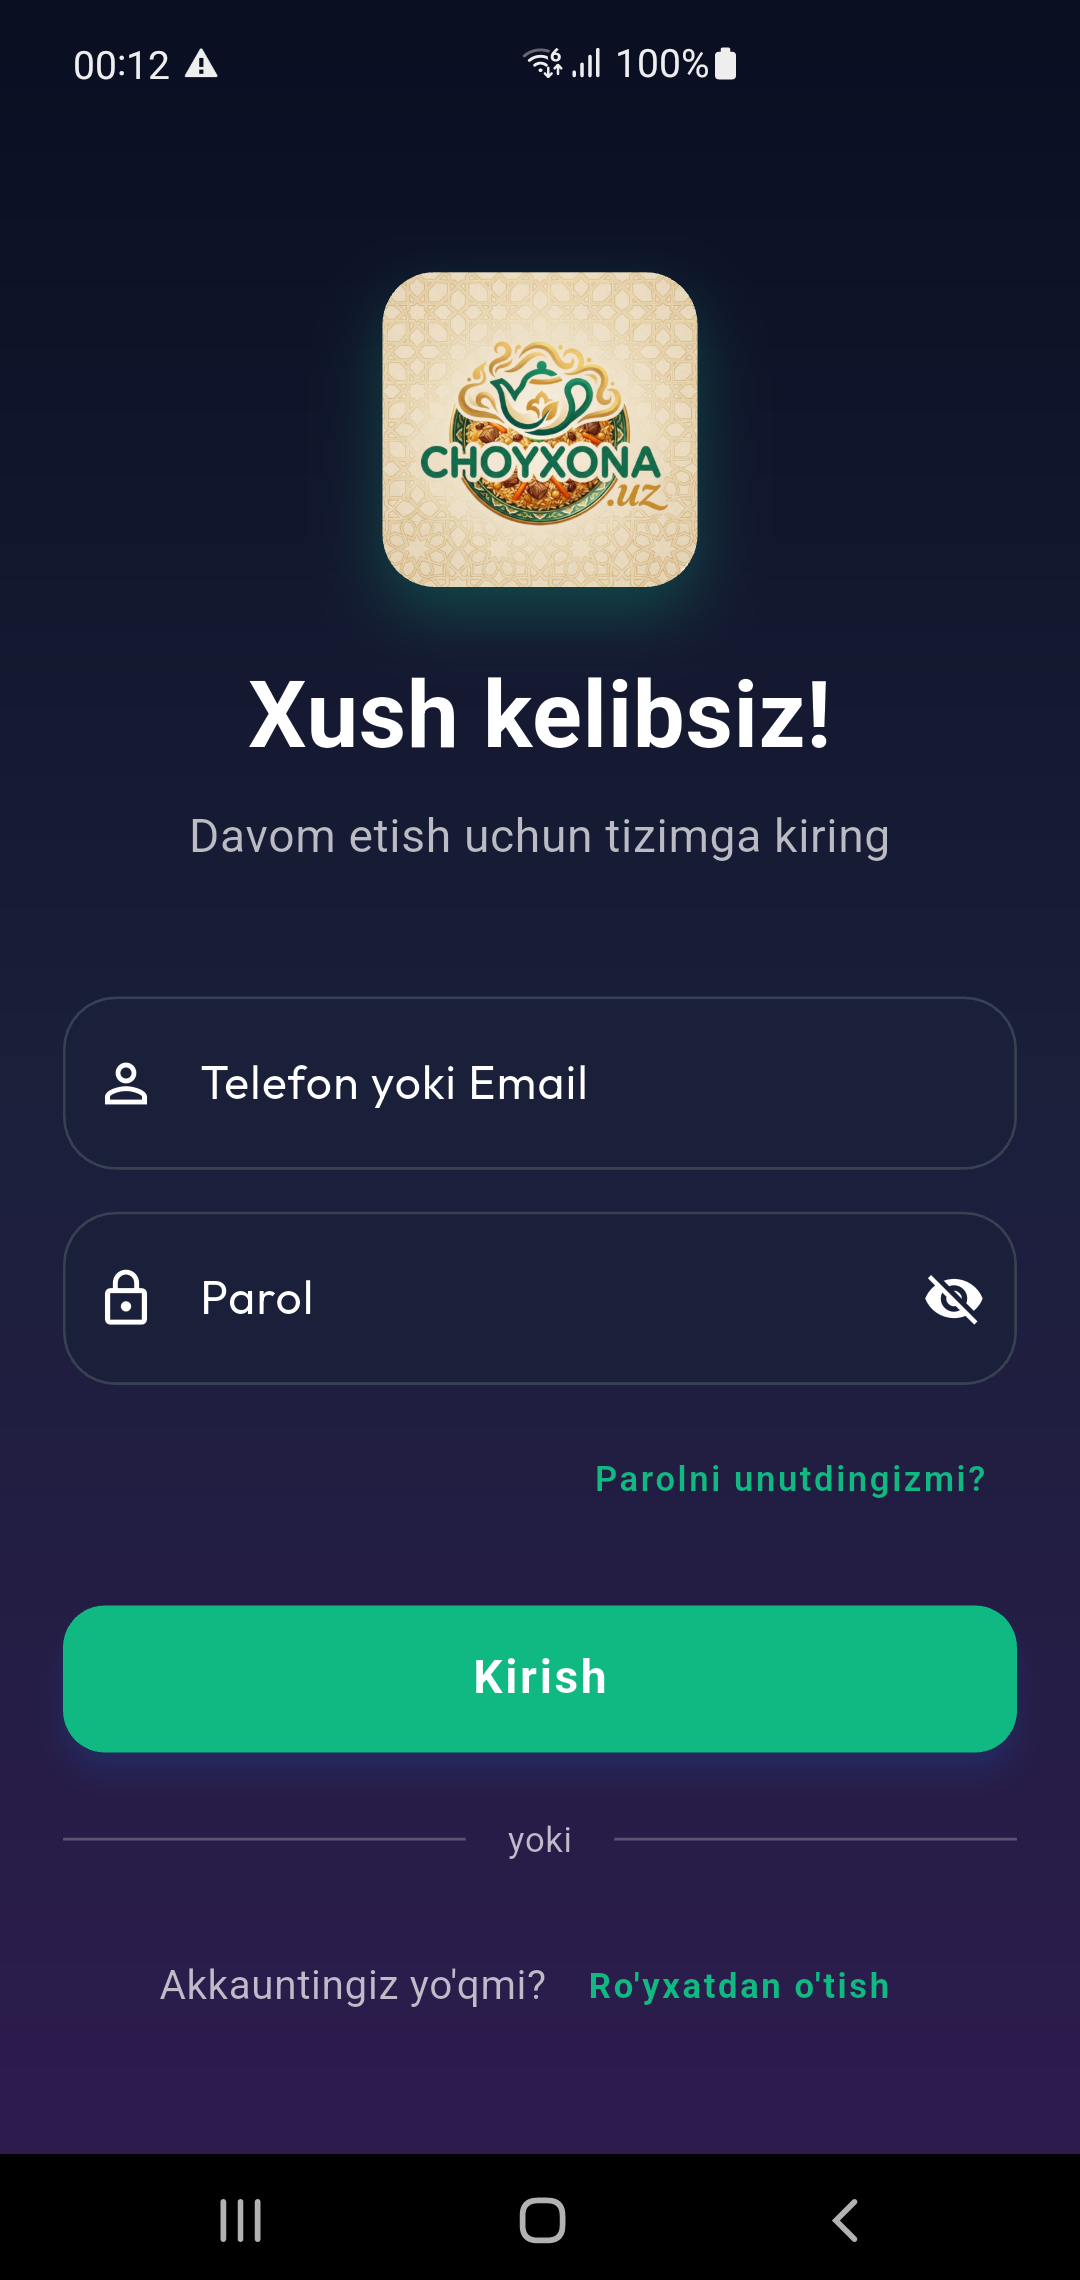
\includegraphics[width=\textwidth]{b_chapters/chapter3/assets/auth_screen.png}
  \end{minipage}
  \hfill
  \begin{minipage}[b]{0.3\textwidth}
    \centering
    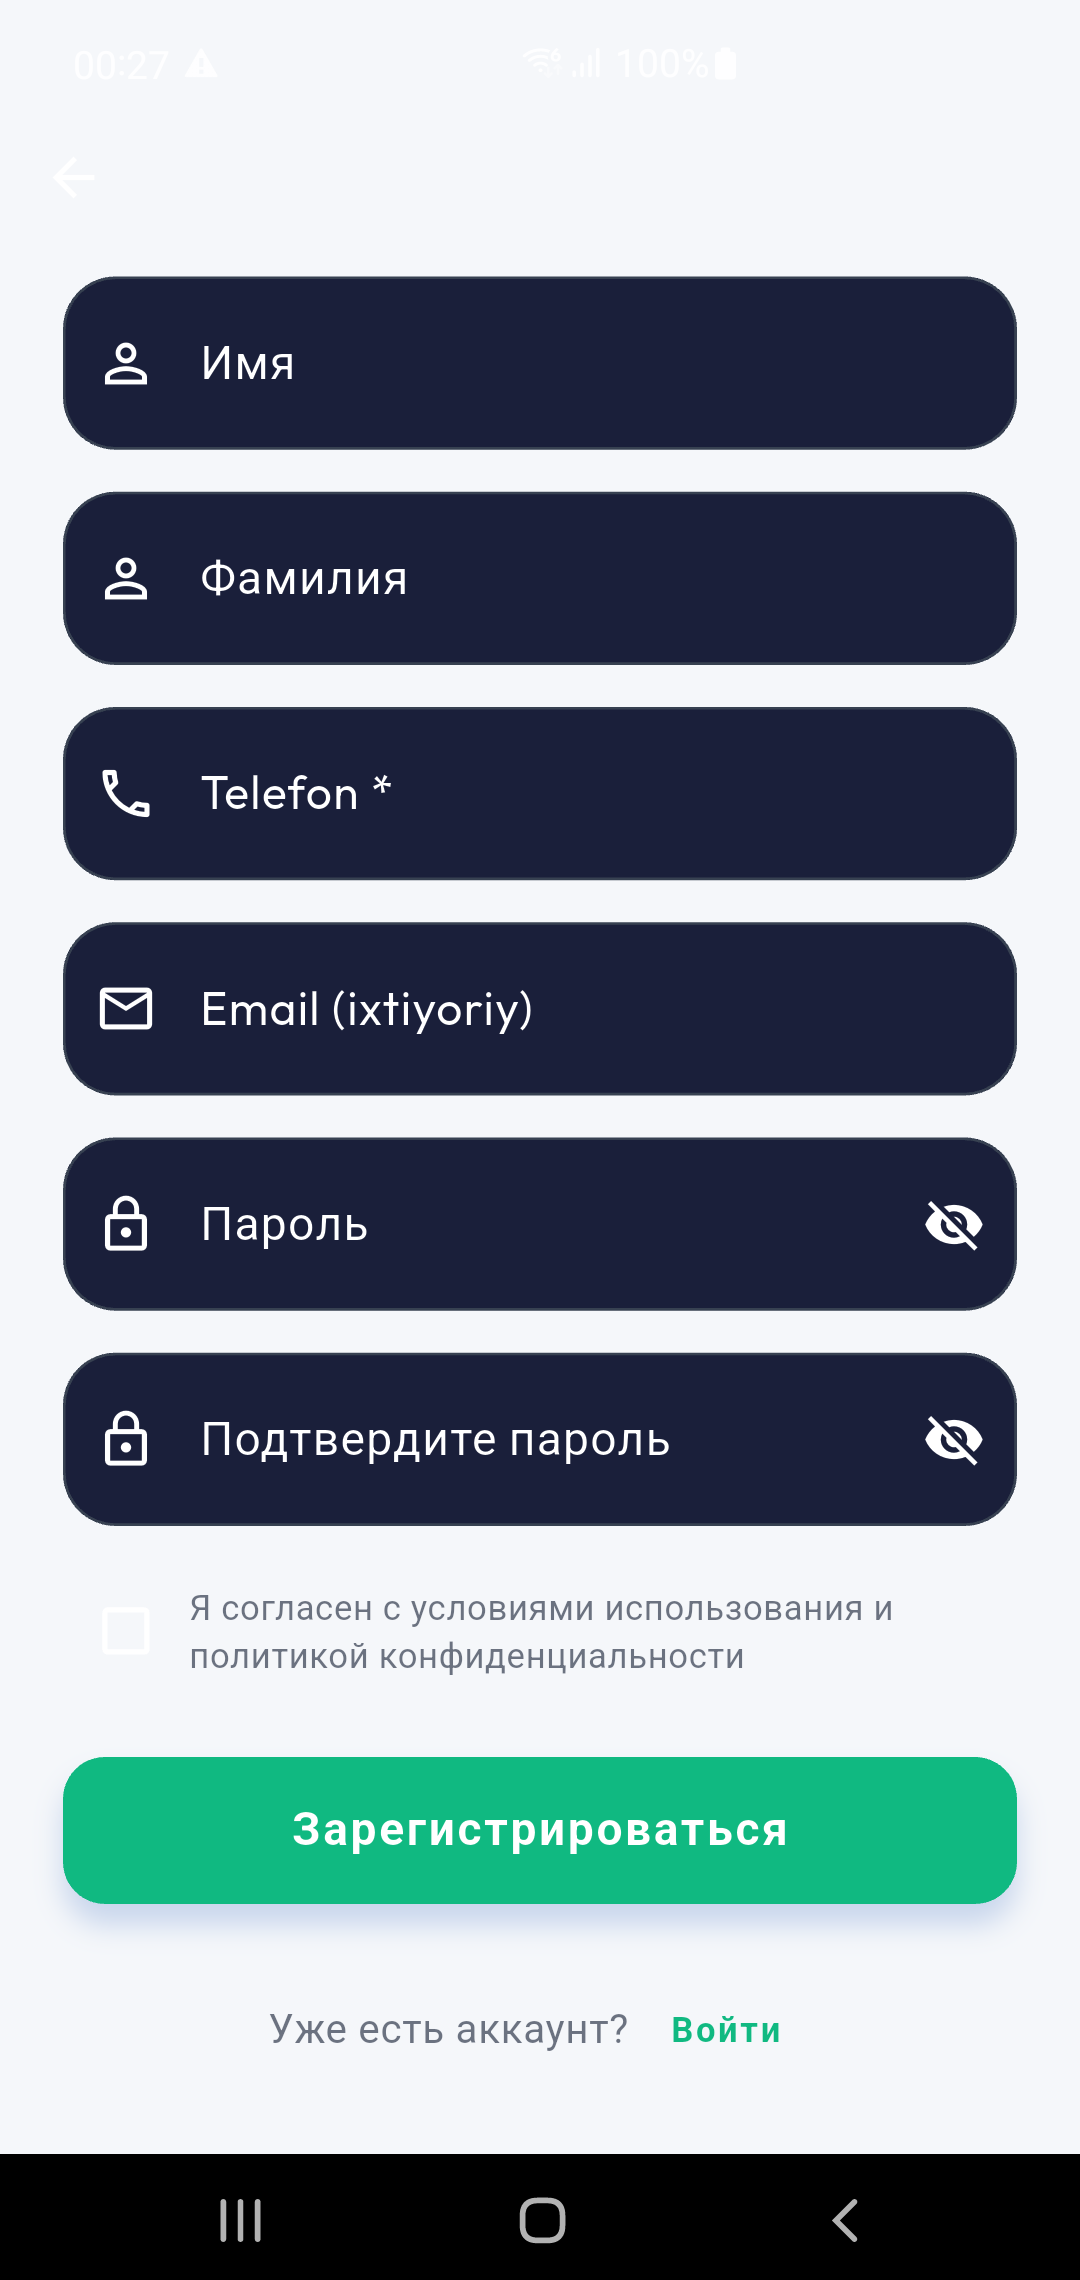
\includegraphics[width=\textwidth]{b_chapters/chapter3/assets/regist_screen.png}
  \end{minipage}
  \figsource{CHOYXONA.UZ application screenshots.}
  \caption{Application flow: splash screen (left), login screen (center), and registration screen (right).}
  \label{fig:splash-auth}
\end{figure}

The \texttt{auth\_service.dart} file encapsulates all Firebase Authentication interactions behind a clean interface, exposing methods including:
\begin{itemize}
  \item \texttt{signInWithEmail()} --- authenticates using email and password credentials;
  \item \texttt{signInWithPhone()} --- initiates and completes phone verification;
  \item \texttt{signOut()} --- ends the session and clears cached data;
  \item \texttt{resetPassword()} --- sends password reset instructions;
  \item \texttt{updatePassword()} --- changes the password for the current user.
\end{itemize}

The \texttt{authStateChanges} stream provides reactive authentication state.
The splash screen subscribes to this stream to determine whether to navigate to the login screen or the main application.
The \texttt{RoleBasedNavigator} component uses authentication state combined with role information to direct users to the appropriate interface~\cite{flutter_state2024}.

\subsection{Role-Based Access Control}
\label{subsec:rbac}

Three primary roles determine feature availability:
\begin{enumerate}
  \item \textbf{User} (customer) --- discovers establishments, makes bookings, and leaves reviews.
  \item \textbf{Admin} (establishment administrator) --- manages a specific establishment; their user document includes an establishment reference.
  \item \textbf{Super Admin} --- oversees the entire platform with access to user management, establishment verification, and system configuration.
\end{enumerate}

Role assignment occurs automatically during registration (as ``user''). Administrator roles are assigned by super administrators through the user management interface.
The role-based routing flow is illustrated in \cref{fig:role-routing}.

\begin{figure}[htbp]
  \centering
  \begin{tikzpicture}[
    box/.style={draw, rounded corners=4pt, minimum width=2.5cm, minimum height=0.8cm, align=center, font=\small, fill=#1!15},
    decision/.style={draw, diamond, aspect=2, minimum width=2cm, inner sep=1pt, font=\small, fill=yellow!10},
    arr/.style={->, thick, >=Stealth},
    node distance=1.2cm
  ]
    \node[box=blue] (splash) {Splash Screen};
    \node[decision, below=of splash] (auth) {Authenticated?};
    \node[box=red, left=2cm of auth] (login) {Login Screen};
    \node[decision, below=of auth] (role) {Role?};
    \node[box=green, below left=1cm and 1.5cm of role] (user) {Customer\\Home};
    \node[box=orange, below=of role] (admin) {Admin\\Dashboard};
    \node[box=purple, below right=1cm and 1.5cm of role] (super) {Super Admin\\Panel};

    \draw[arr] (splash) -- (auth);
    \draw[arr] (auth) -- node[above,font=\scriptsize]{No} (login);
    \draw[arr] (auth) -- node[right,font=\scriptsize]{Yes} (role);
    \draw[arr] (role) -- node[left,font=\scriptsize]{user} (user);
    \draw[arr] (role) -- node[right,font=\scriptsize]{admin} (admin);
    \draw[arr] (role) -- node[right,font=\scriptsize]{superadmin} (super);
    \draw[arr] (login.south) |- ++(0,-0.5) -| (auth);
  \end{tikzpicture}
  \caption{Role-based navigation routing from splash screen to role-specific interfaces.}
  \label{fig:role-routing}
\end{figure}

\subsection{Profile Management and Security}
\label{subsec:profile-security}

The profile management screen enables users to view and update personal information: profile photo (with camera capture or gallery selection, compressed before upload to Cloud Storage), display name, phone number (requiring re-verification), language preference, and notification settings.
Preferences synchronize across devices through Firestore~\cite{firebase_firestore2024}.

Security considerations include: passwords never stored locally (only session tokens managed by Firebase SDK), sensitive operations requiring recent authentication, rate limiting on Firebase servers preventing brute-force attacks, and automatic account lockout after repeated failed attempts~\cite{firebase_auth2024}.


% =====================================================================
\section{Search, Filtering, and Booking Process}
\label{sec:search-booking}

The discovery and booking flow represents the core user journey, taking users from initial exploration through confirmed reservation.

\subsection{Discovery and Search}
\label{subsec:discovery}

The \textbf{home screen} combines curated content with personalized recommendations.
A search bar provides quick text access, a horizontal carousel displays featured establishments, and personalized recommendations appear based on user history~\cite{nielsen2012}.

The \textbf{search screen} offers comprehensive multi-dimensional filtering:

\begin{table}[htbp]
\caption{Search filter dimensions and available options}
\label{tab:search-filters}
\centering
\small
\begin{tabular}{lp{8cm}}
\toprule
\textbf{Filter} & \textbf{Options} \\
\midrule
Text search     & Name, description, and tag matching \\
Category        & Traditional teahouse, National cuisine, European, Mixed menu \\
Price range     & Budget-friendly ($), Moderate (\$\$), Upscale (\$\$\$) \\
Rating          & Minimum 3 stars, Minimum 4 stars \\
Location        & Region dropdown (Tashkent, Samarkand, Bukhara, etc.) \\
Distance        & Radius from current location (requires GPS permission) \\
Sorting         & Relevance, Distance, Rating, Newest \\
\bottomrule
\end{tabular}
\end{table}

Results display as scrollable \texttt{ChoyxonaCard} widgets with establishment image, name, star rating with review count, price indicator, and distance.
The list supports infinite scroll with lazy loading.
The customer-facing interface is shown in \cref{fig:user-interface}.

\begin{figure}[htbp]
  \centering
  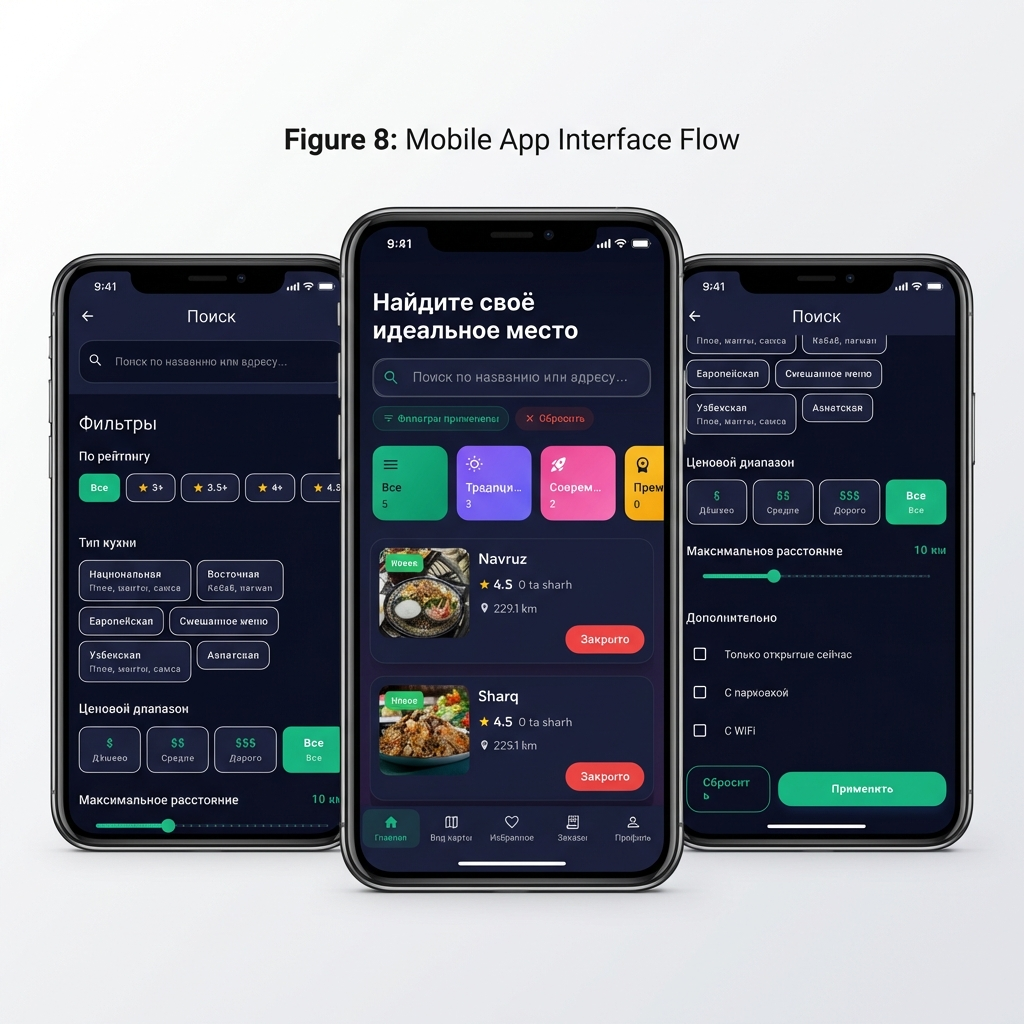
\includegraphics[width=0.7\textwidth]{b_chapters/chapter3/assets/user_collage.png}
  \figsource{CHOYXONA.UZ application screenshots.}
  \caption{Customer interface overview: home screen with featured establishments, search results, and establishment detail view.}
  \label{fig:user-interface}
\end{figure}

The \textbf{establishment detail screen} organizes information into tabbed sections: Overview (description, amenities, features), Menu (food and beverage with photos, prices, and categories loaded from subcollection), and Reviews (user feedback with ratings and text, sorted by recency or helpfulness).

\subsection{Booking Process}
\label{subsec:booking-process}

The booking process guides users through a structured four-step flow, as shown in \cref{fig:booking-flow}.

\begin{figure}[htbp]
  \centering
  \begin{minipage}[b]{0.3\textwidth}
    \centering
    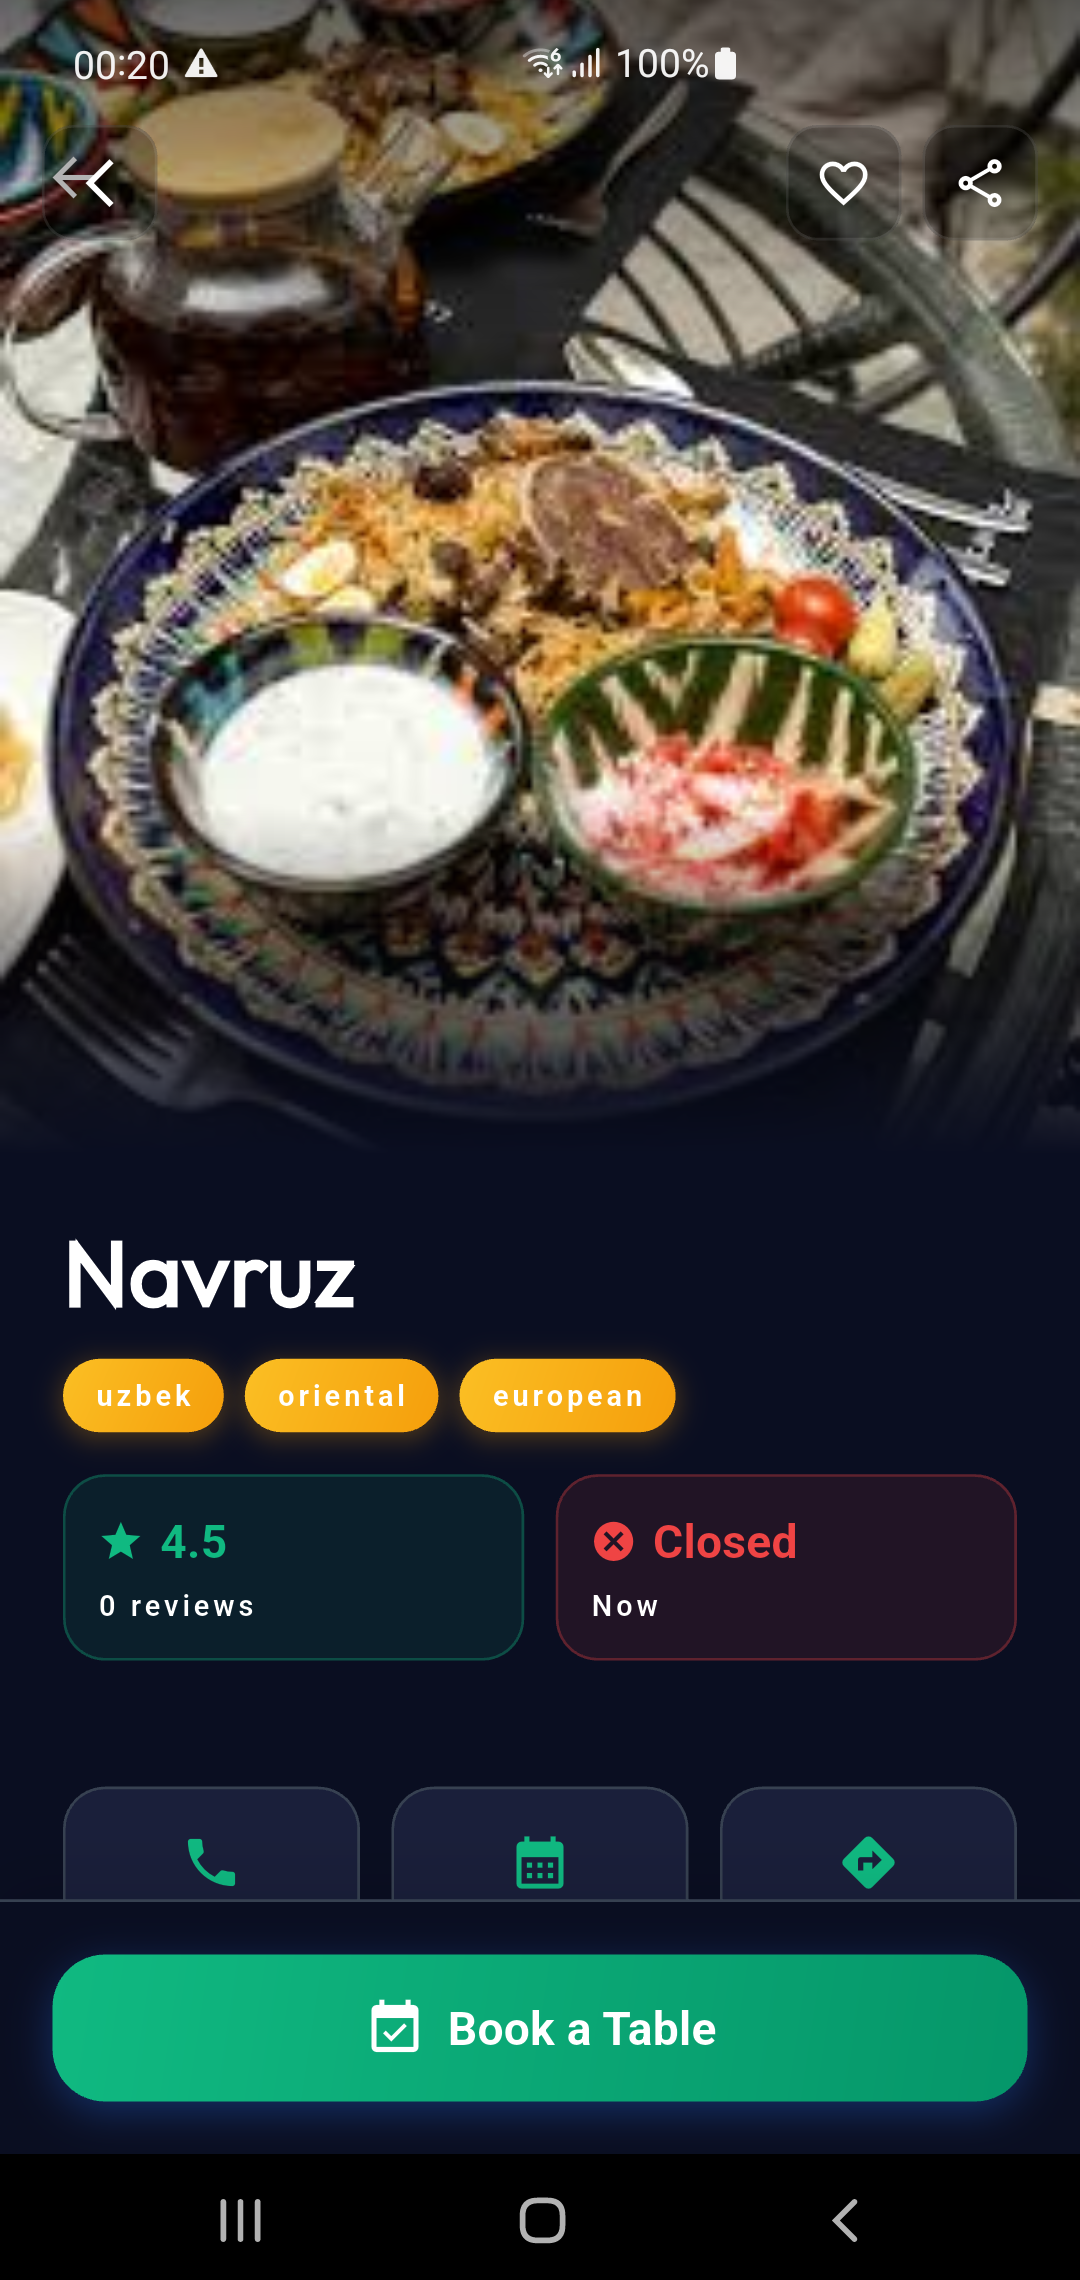
\includegraphics[width=\textwidth]{b_chapters/chapter3/assets/booking_step1.png}
  \end{minipage}
  \hfill
  \begin{minipage}[b]{0.3\textwidth}
    \centering
    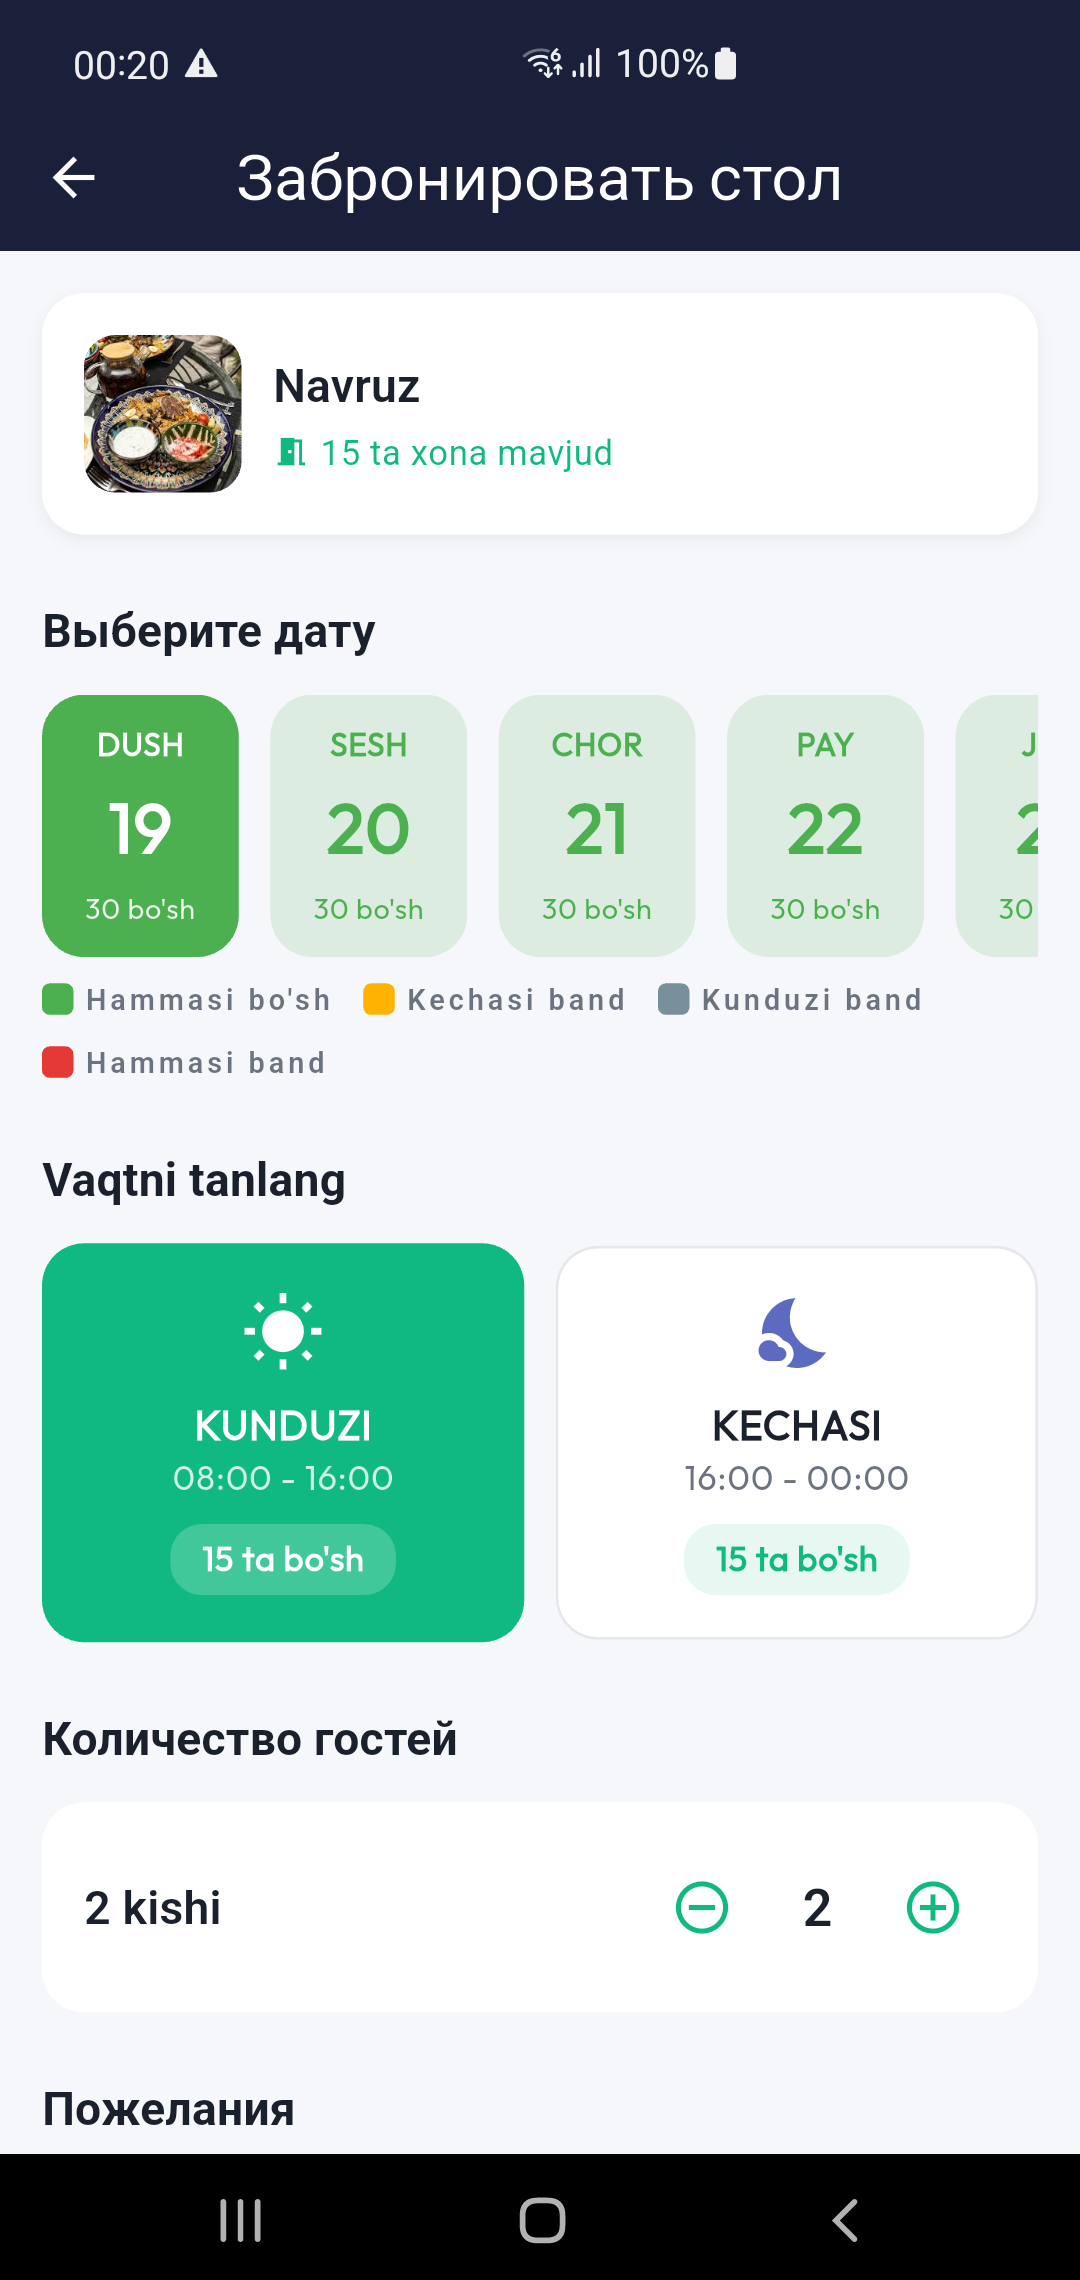
\includegraphics[width=\textwidth]{b_chapters/chapter3/assets/booking_step2.png}
  \end{minipage}
  \hfill
  \begin{minipage}[b]{0.3\textwidth}
    \centering
    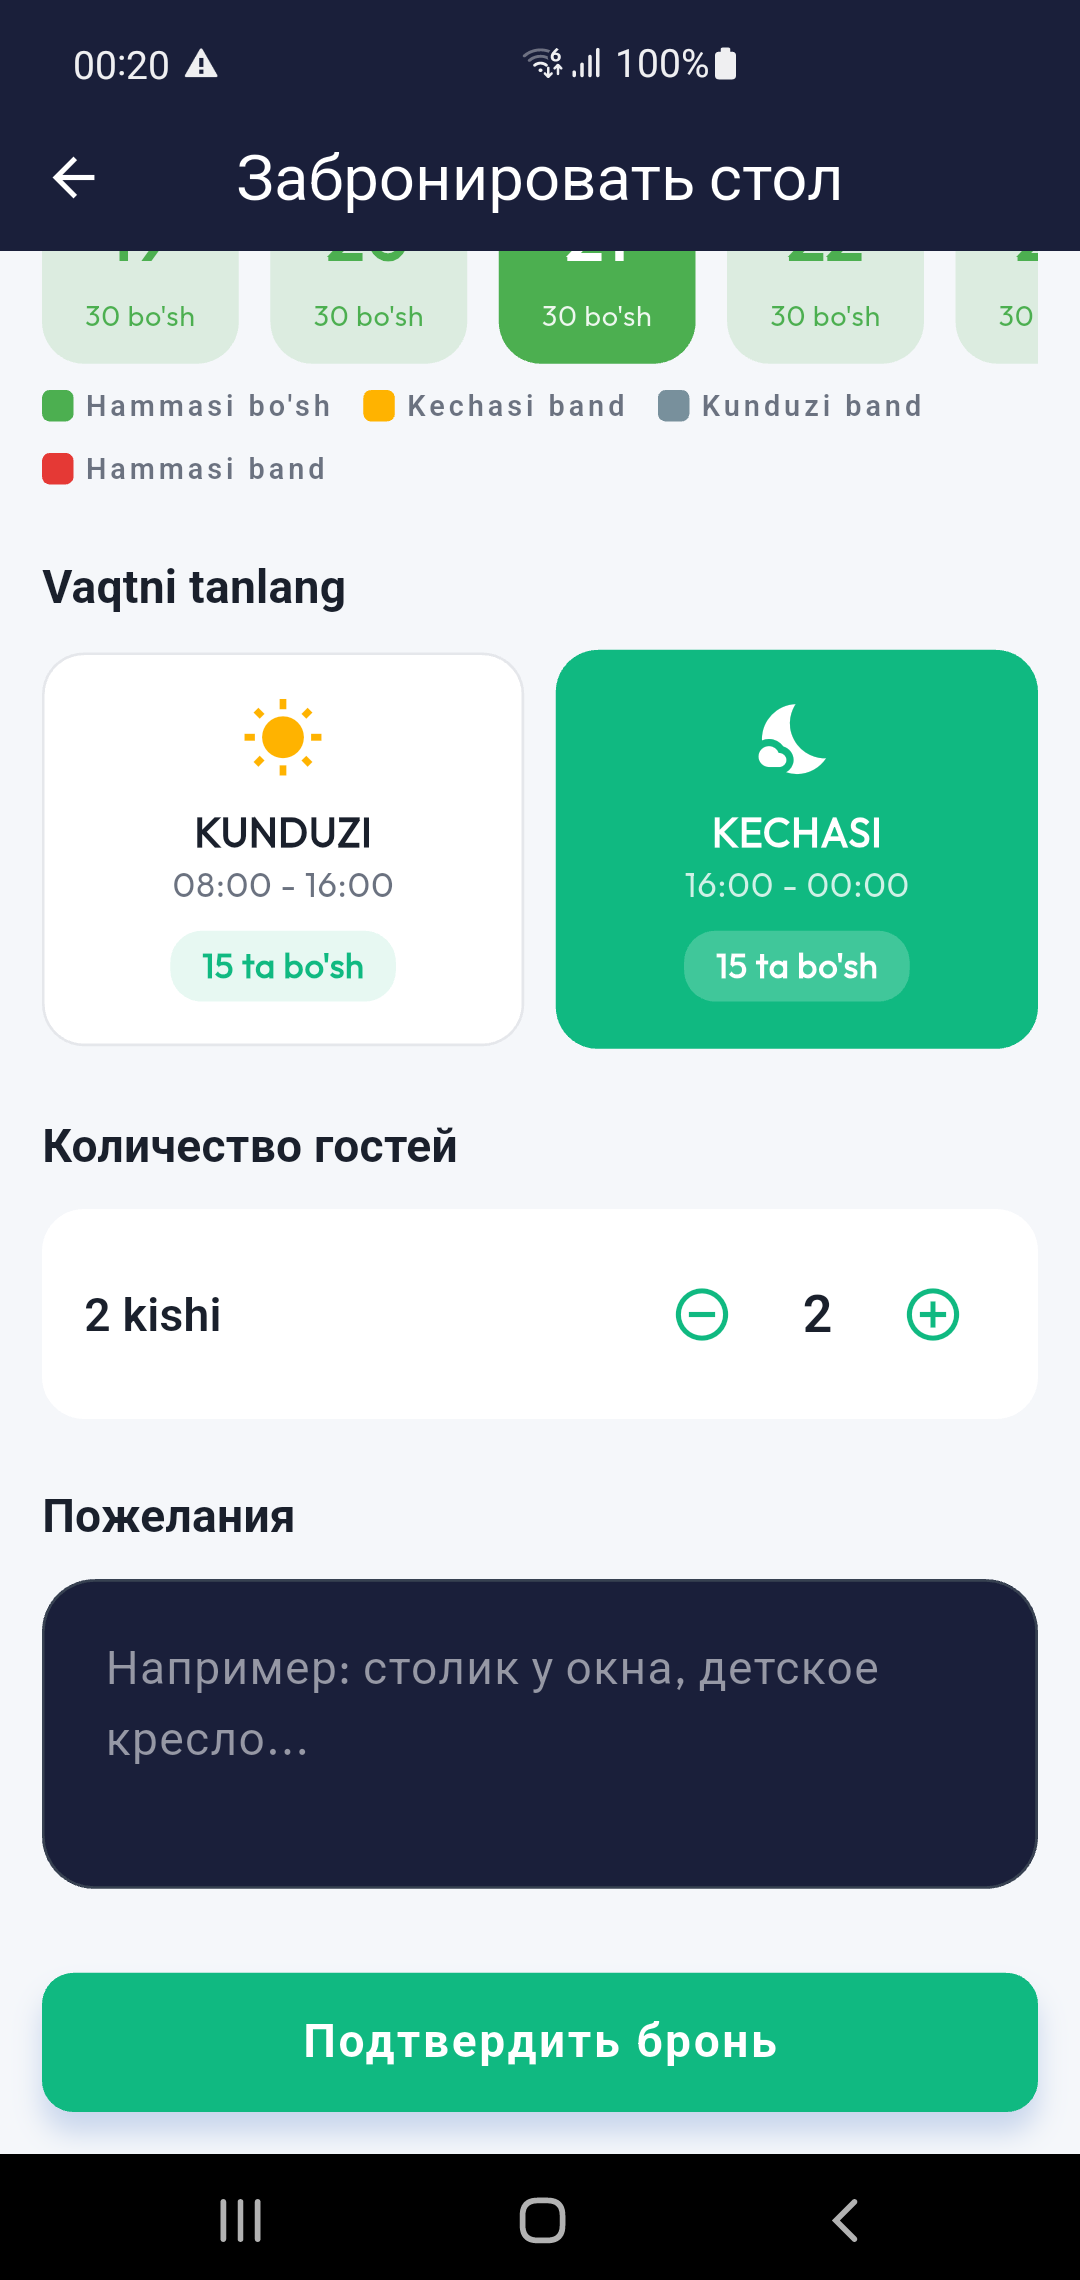
\includegraphics[width=\textwidth]{b_chapters/chapter3/assets/booking_step3.png}
  \end{minipage}
  \figsource{CHOYXONA.UZ application screenshots.}
  \caption{Booking process: date and time selection (left), party details and room preference (center), and booking confirmation (right).}
  \label{fig:booking-flow}
\end{figure}

The booking steps are:

\textbf{Step~1: Date selection.}
A calendar interface highlights dates with available slots while dimming fully booked dates.
Users cannot select past dates or dates beyond the establishment's advance booking window.

\textbf{Step~2: Time slot selection.}
Available slots for the chosen date display as tappable buttons with color-coded availability: green (fully available), yellow (limited availability), hidden (fully booked).
Slots are generated based on the establishment's configured duration and capacity.

\textbf{Step~3: Party details and room preference.}
A numeric stepper adjusts guest count within the establishment's limits.
For establishments offering private rooms (\textit{xona}), available room options show name, capacity, fee, and thumbnail.
Users can select a specific room or indicate no preference.

\textbf{Step~4: Confirmation.}
A summary of all selections appears for review.
Users can add special requests (dietary requirements, celebrations, seating preferences).
Cancellation policy terms require acknowledgment via checkbox~\cite{sommerville2015}.

Upon confirmation, the booking is submitted through a \textbf{Firestore transaction} that atomically verifies availability and creates the booking document.
If a conflict exists, the user is returned to time selection.
Successful bookings generate a unique reference code and QR code for quick check-in.
A push notification confirms the reservation immediately~\cite{firebase_firestore2024}.

\textbf{Booking management} enables users to view (upcoming/past sections), cancel (with reason prompt), or modify reservations.
A ``book again'' feature pre-fills details from previous visits for convenience.


% =====================================================================
\section{Administrator Panel}
\label{sec:admin-panel}

Establishment administrators access specialized management tools through a dedicated dashboard, as shown in \cref{fig:admin-dashboard}.

\begin{figure}[htbp]
  \centering
  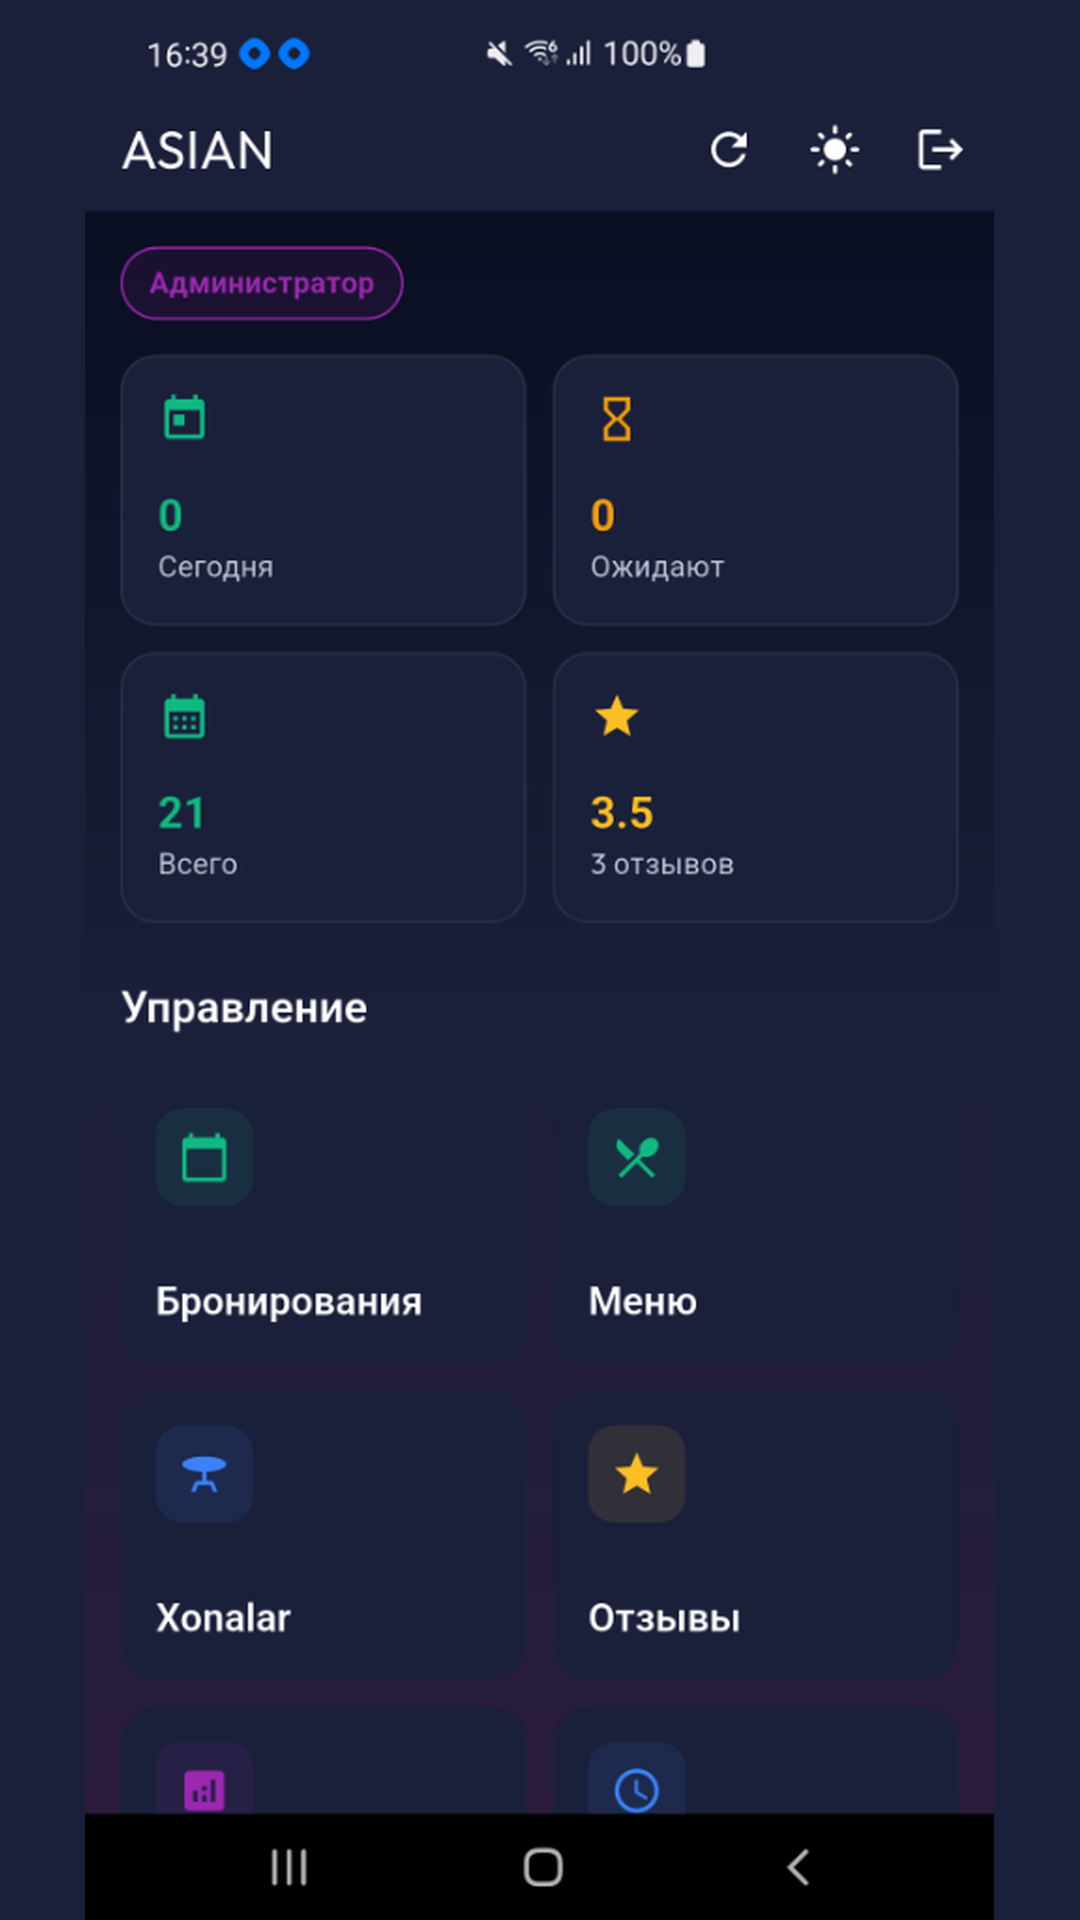
\includegraphics[width=0.4\textwidth]{b_chapters/chapter3/assets/admin_dashboard.png}
  \figsource{CHOYXONA.UZ application screenshot.}
  \caption{Administrator dashboard displaying key performance indicators: today's bookings, pending reservations, total bookings, and average rating.}
  \label{fig:admin-dashboard}
\end{figure}

\subsection{Dashboard and Key Metrics}
\label{subsec:admin-dashboard}

The dashboard home presents key performance indicators (KPIs) at a glance:
\begin{itemize}
  \item \textbf{Today's bookings} --- count with status breakdown (confirmed, pending, checked in, completed);
  \item \textbf{Pending actions} --- items requiring attention (booking confirmations, review responses);
  \item \textbf{Capacity utilization} --- current bookings versus available capacity;
  \item \textbf{Average rating} --- establishment rating with review count;
  \item \textbf{Total bookings} --- cumulative reservation count.
\end{itemize}

Trend indicators compare current values to previous periods (same day last week, monthly averages).
Quick action buttons provide single-tap access to common tasks: view today's schedule, confirm pending bookings, or create a new promotion~\cite{wasserman2010}.

\subsection{Booking and Calendar Management}
\label{subsec:booking-mgmt}

The \textbf{calendar view} provides monthly booking pattern overview with color-coded density cells (light for few, medium for moderate, dark for heavily booked days).
Selecting a day reveals a detailed timeline where bookings appear as positioned blocks with customer name, party size, and room assignment.
Color coding indicates status: blue (confirmed), green (checked in), gray (completed), red (cancelled/no-show).

Booking management capabilities include:
\begin{itemize}
  \item \textbf{Confirmation} --- reviewing and approving new booking requests;
  \item \textbf{Modification} --- adjusting party size, time, or room assignment with audit logging;
  \item \textbf{Cancellation} --- with reason recording and automated customer notification;
  \item \textbf{Check-in/Check-out} --- via QR code scanning or manual search, recording arrival time and actual party size.
\end{itemize}

\subsection{Reports, Analytics, and Menu Management}
\label{subsec:reports-menu}

The \textbf{reports screen} presents analytical views through charts and summary metrics:

\begin{table}[htbp]
\caption{Administrator analytics categories and metrics}
\label{tab:admin-analytics}
\centering
\small
\begin{tabular}{lp{8cm}}
\toprule
\textbf{Category} & \textbf{Metrics} \\
\midrule
Revenue      & Daily totals (line/bar charts), period comparison, estimated from party sizes $\times$ avg.\ check \\
Bookings     & Peak hour distribution, day-of-week patterns, lead time analysis, cancellation rate trends \\
Customers    & New vs.\ returning breakdown, party size distribution, geographic analysis \\
Reviews      & Average rating trend, sentiment indicators, response rate \\
\bottomrule
\end{tabular}
\end{table}

\textbf{Menu management} allows adding items (name, description, price, category, photo), editing, and marking items as temporarily unavailable.
Changes synchronize immediately through Firestore real-time updates.
\textbf{Promotion management} enables creating special offers with title, description, discount details, validity period, and customer targeting~\cite{firebase_firestore2024}.


% =====================================================================
\section{Super Admin Panel and Platform Oversight}
\label{sec:superadmin}

Super administrators oversee the entire CHOYXONA.UZ platform with responsibilities spanning user management, establishment verification, content moderation, and system configuration.
The super admin interface is shown in \cref{fig:superadmin-panel}.

\begin{figure}[htbp]
  \centering
  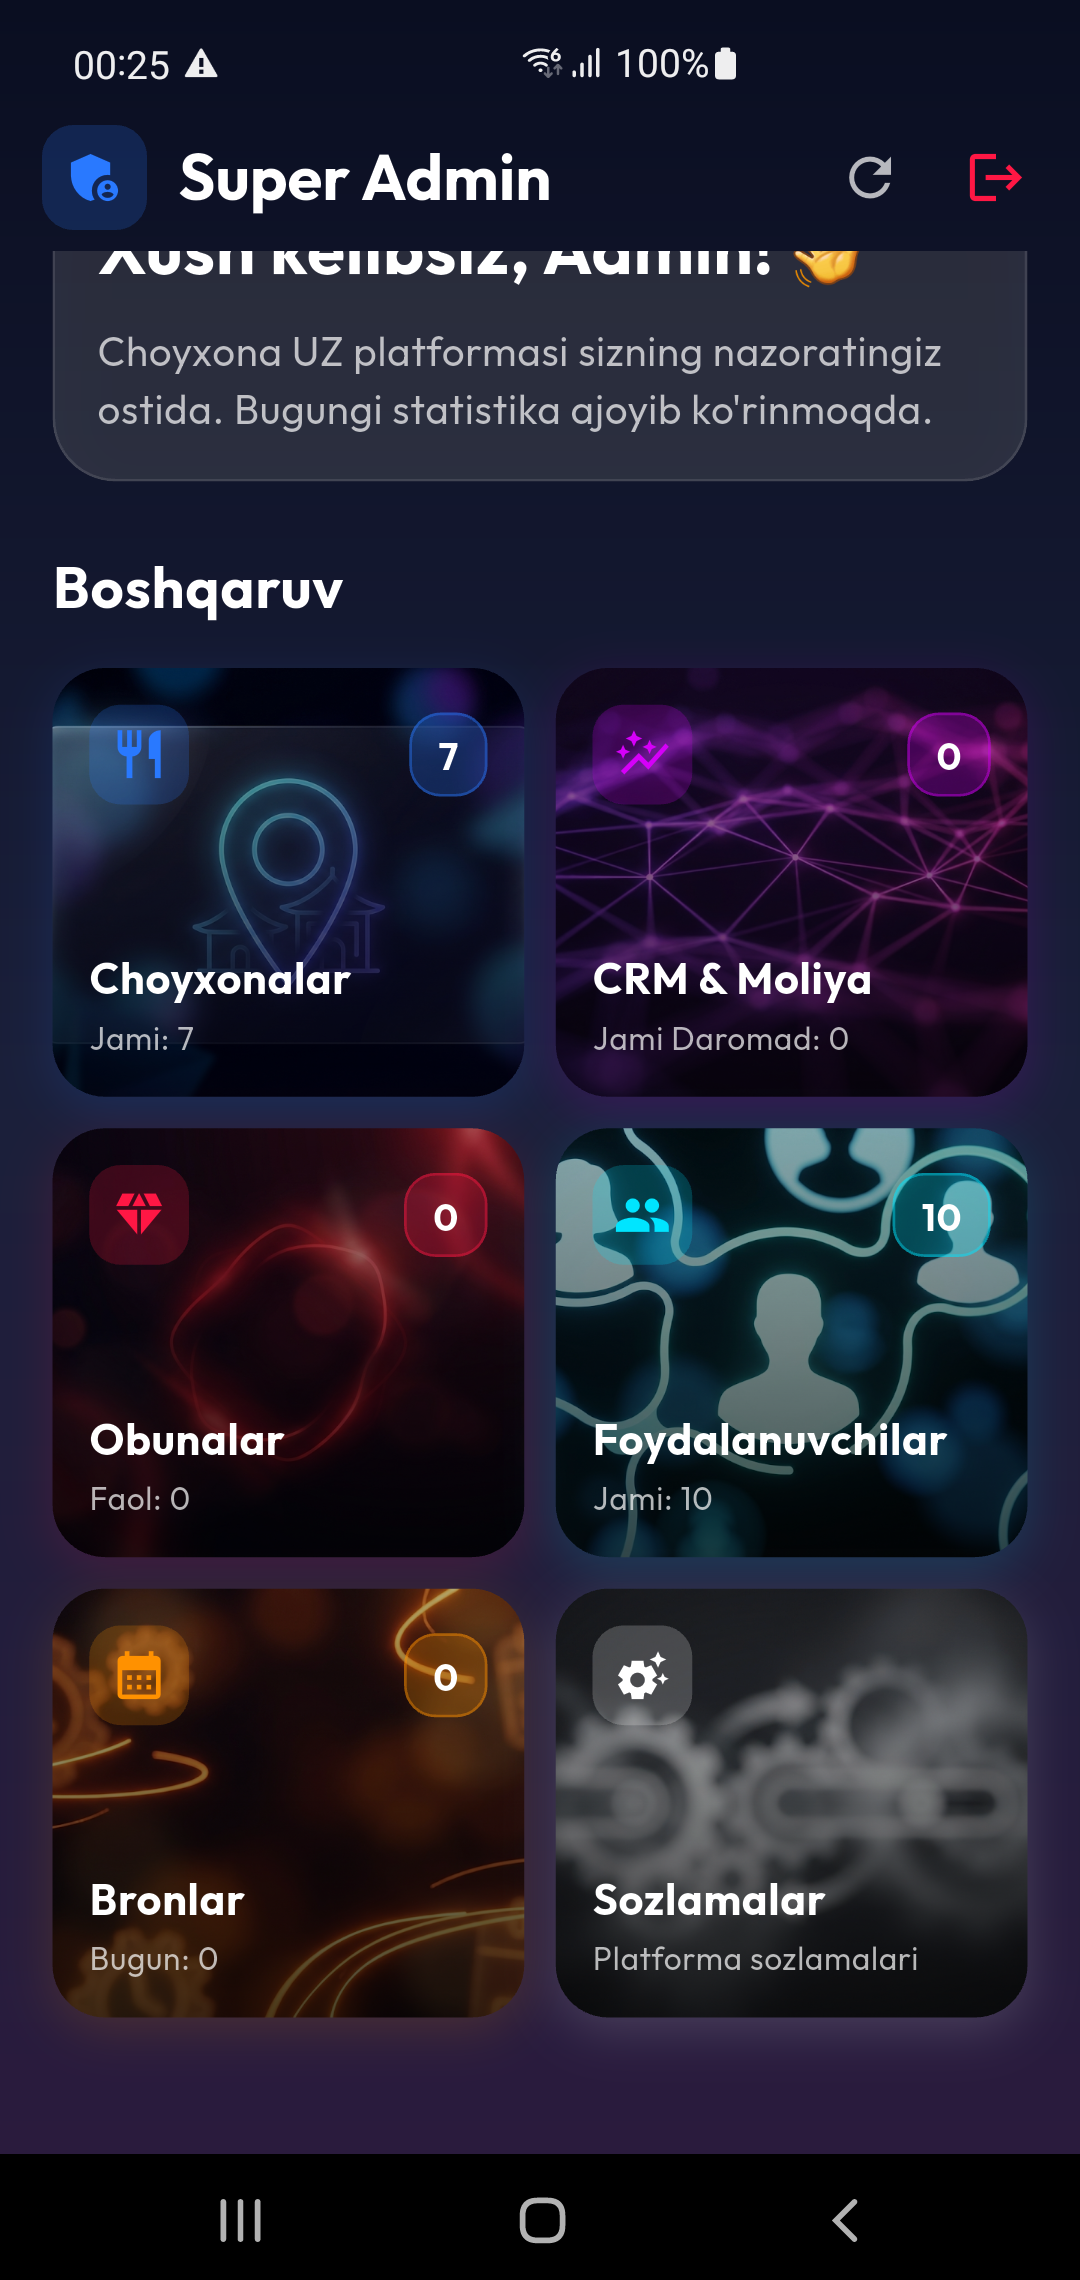
\includegraphics[width=0.4\textwidth]{b_chapters/chapter3/assets/superadmin.png}
  \figsource{CHOYXONA.UZ application screenshot.}
  \caption{Super administrator control panel showing platform-wide management capabilities and monitoring tools.}
  \label{fig:superadmin-panel}
\end{figure}

\subsection{Platform Metrics and Verification}
\label{subsec:platform-metrics}

The super admin dashboard presents platform-wide metrics: total registered users with growth trend, active establishments by region, total processed bookings, and system health indicators.
Growth charts visualize user registration trends, establishment onboarding, and booking volume over time~\cite{jia2014}.

The \textbf{establishment verification workflow} ensures quality of listed businesses:
\begin{enumerate}
  \item New establishments enter \textit{pending} state (invisible to users);
  \item Verification queue shows submitted information and documentation;
  \item Super admin reviews information for completeness and authenticity;
  \item Approval makes establishment visible in search; rejection sends corrective feedback;
  \item Premium verification badges may involve additional steps including in-person visits.
\end{enumerate}

\subsection{User Management and Content Moderation}
\label{subsec:user-management}

User management provides oversight of all registered accounts with search, filtering by role/date/activity, and detailed profile views.
Available moderation actions include:

\begin{itemize}
  \item \textbf{Role modification} --- granting or revoking administrator access;
  \item \textbf{Warning issuance} --- for policy violations (recorded and visible to user);
  \item \textbf{Suspension} --- temporary sign-in prevention during investigations;
  \item \textbf{Permanent ban} --- for severe violations (prevents future registration).
\end{itemize}

Each action logs the super administrator, reason, and timestamp for accountability~\cite{martin2017}.

Content moderation addresses reported reviews through a queue with dismiss/remove/warn options.
Automated keyword filtering flags potentially problematic content for prioritized review.

\subsection{System Configuration}
\label{subsec:system-config}

System configuration enables adjustments without code deployment:
\begin{itemize}
  \item \textbf{Feature flags} --- staged rollout of new functionality to user subsets;
  \item \textbf{Configuration values} --- default search radius, max booking days, min review length;
  \item \textbf{Featured content} --- home screen carousel, promotional banners, announcements.
\end{itemize}

Configurations are stored in a dedicated Firestore collection and loaded by clients during initialization~\cite{firebase_functions2024}.


% =====================================================================
\section{Notification System}
\label{sec:notifications}

The notification system maintains user engagement and delivers timely information throughout the customer journey~\cite{firebase_functions2024}.

Firebase Cloud Messaging (FCM) powers push notifications on both Android and iOS.
The \texttt{PushNotificationService} class manages the complete lifecycle: permission request, device token retrieval and storage, token refresh handling, and notification delivery~\cite{khawas2018}.

Notification categories serve distinct purposes, as summarized in \cref{tab:notification-types}.

\begin{table}[htbp]
\caption{Notification categories, priorities, and trigger conditions}
\label{tab:notification-types}
\centering
\small
\begin{tabular}{llp{5.5cm}}
\toprule
\textbf{Category} & \textbf{Priority} & \textbf{Trigger and Content} \\
\midrule
Booking confirmation & High   & Immediately after reservation: establishment, date, time, reference \\
Reminder (24h)       & Medium & 24 hours before booking \\
Reminder (2h)        & Medium & 2 hours before booking \\
Promotional          & Low    & Special offers from favorited establishments (user-configurable) \\
System               & Low    & Platform announcements, maintenance, new features \\
\bottomrule
\end{tabular}
\end{table}

Notification behavior adapts to application state: \textbf{foreground} notifications display as in-app snackbar overlays; \textbf{background/terminated} notifications appear in the device notification shade and navigate to relevant content on tap.

The notification center (\cref{fig:notifications}) provides persistent history with unread indicators and mark-all-read functionality.

\begin{figure}[htbp]
  \centering
  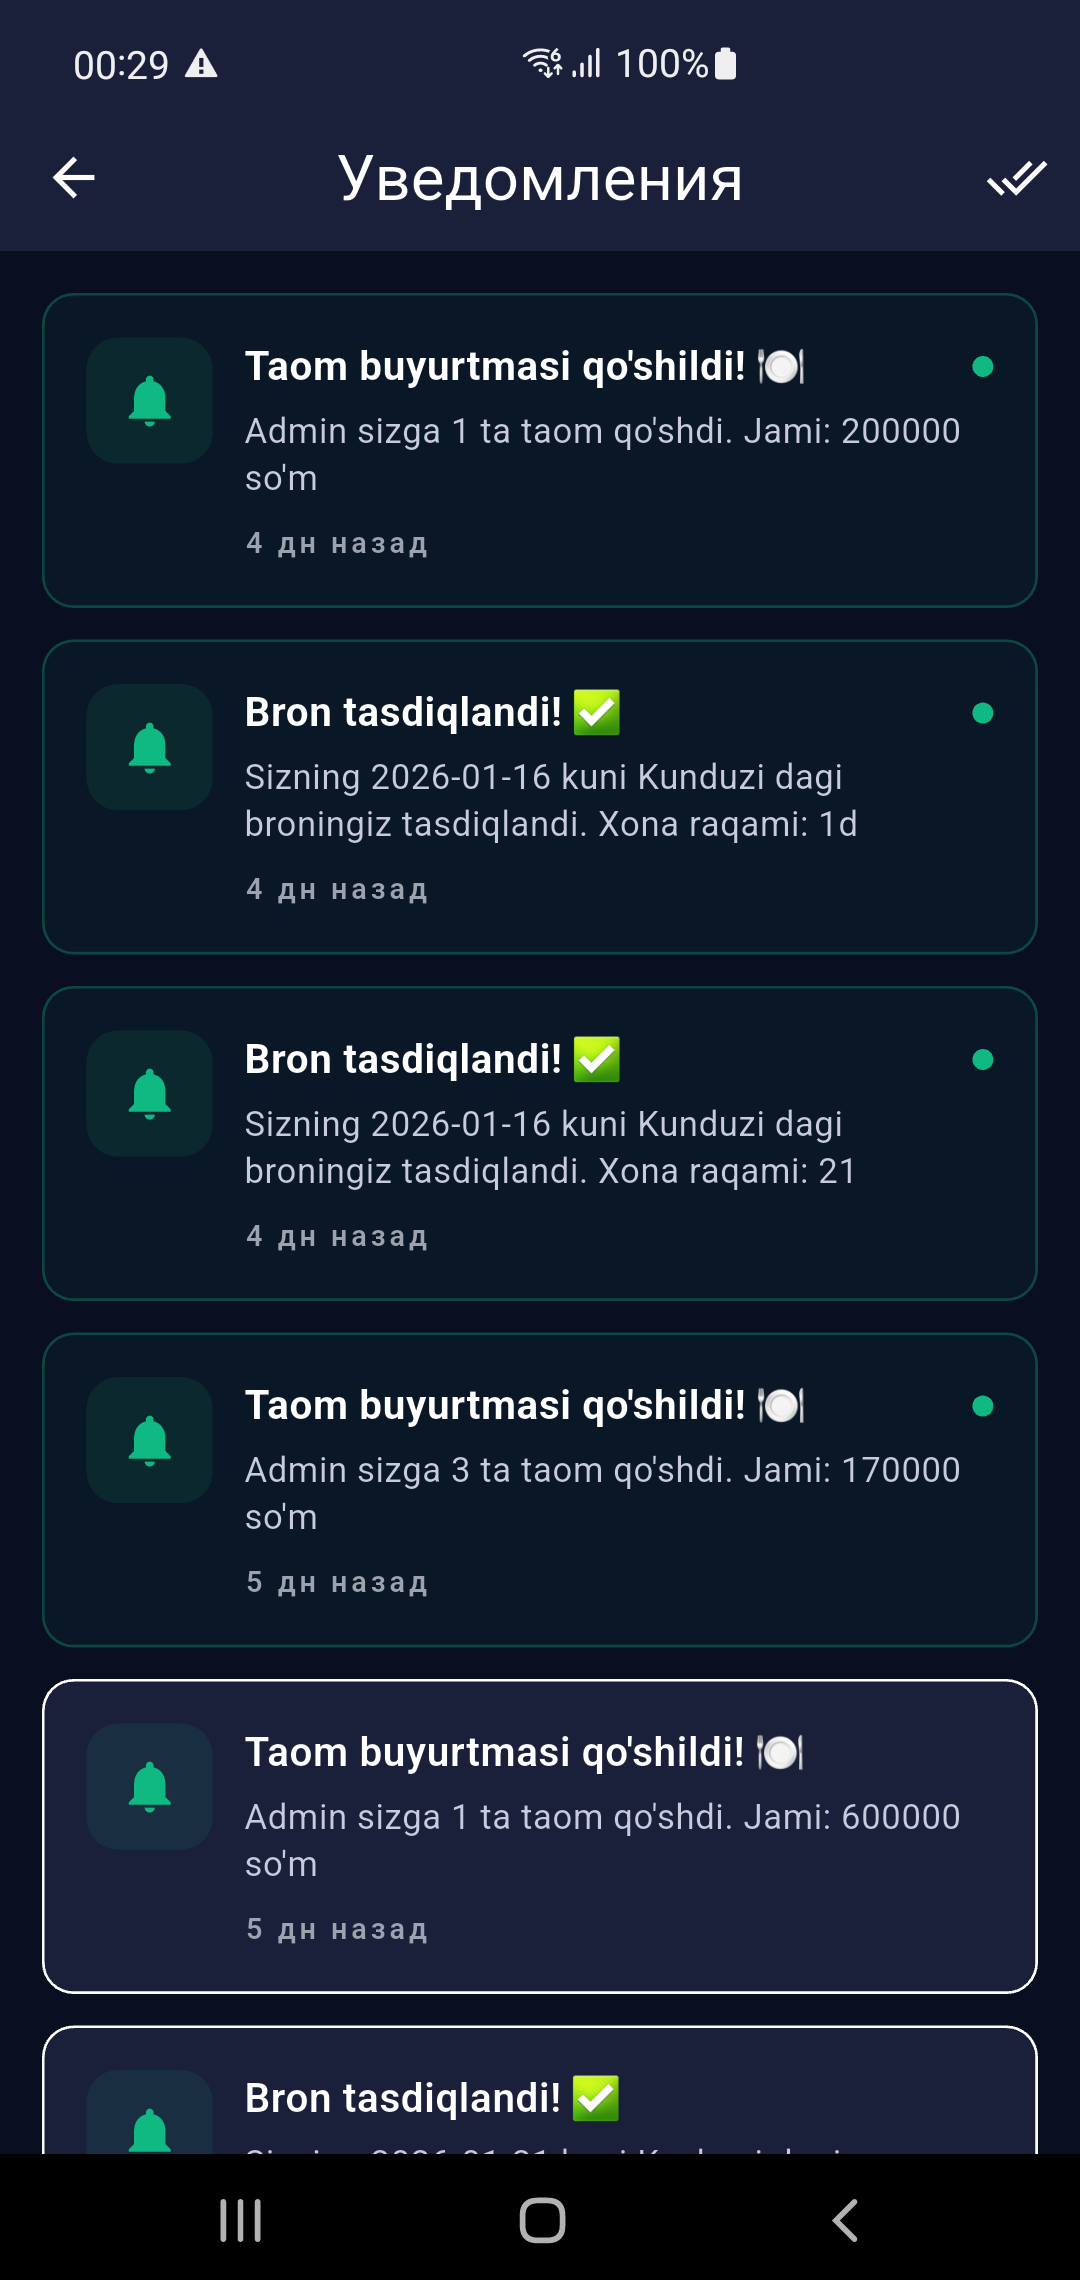
\includegraphics[width=0.4\textwidth]{b_chapters/chapter3/assets/notifications.png}
  \figsource{CHOYXONA.UZ application screenshot.}
  \caption{Notification center displaying booking confirmations, reminders, and system messages with unread indicators.}
  \label{fig:notifications}
\end{figure}

The notification preferences screen provides granular control: independent category toggles and quiet hours configuration.
Preferences update immediately in Firestore~\cite{firebase_firestore2024}.


% =====================================================================
\section{Chapter Summary}
\label{sec:ch3-summary}

This chapter demonstrated the complete functional capabilities of CHOYXONA.UZ through its three user roles:

First, \cref{sec:user-module} described the authentication module supporting email/password and phone/SMS methods (\cref{fig:splash-auth}), role-based access control routing users to appropriate interfaces (\cref{fig:role-routing}), and profile management with cross-device synchronization.

Second, \cref{sec:search-booking} detailed the core customer journey from discovery through booking confirmation.
The multi-dimensional search system (\cref{tab:search-filters}) enables precise establishment matching, while the four-step booking flow (\cref{fig:booking-flow}) guides users through date, time, party, and room selection with transactional consistency ensuring no double-bookings.

Third, \cref{sec:admin-panel} presented the administrator dashboard (\cref{fig:admin-dashboard}) with KPIs, calendar-based booking management, analytics (\cref{tab:admin-analytics}), menu management, and promotion tools.

Fourth, \cref{sec:superadmin} covered the super administrator panel (\cref{fig:superadmin-panel}) providing platform oversight through establishment verification workflows, user management with moderation actions, content moderation, and remote system configuration.

Fifth, \cref{sec:notifications} described the FCM-based notification system with five categories (\cref{tab:notification-types}), adaptive behavior based on application state, and user-configurable preferences.

These functional capabilities collectively deliver a comprehensive three-sided marketplace connecting customers, establishment administrators, and platform operators.
The testing and deployment of this implementation are addressed in Chapter~4.
